\documentclass{article}
\usepackage[utf8]{inputenc}
\usepackage{graphicx, graphics, float}
\usepackage[a4paper, total={6in, 9in}]{geometry}
\usepackage[spanish]{babel}
\usepackage{subcaption}
\title{Haz Una Línea\\
\large Memoria DS - Práctica 3}
\author{Andrés Merlo Trujillo\\ Sergio Hervás Cobo\\ Javier Serrano Lucas\\ Ricardo Molina Rodríguez}

\begin{document}
\date{Abril 2022}
\maketitle
\section{Introducción}
En esta práctica se ha realizado una serie de pruebas para comprobar el funcionamiento correcto de
ciertas funcionalidades y métodos de la aplicación realizada en la Práctica 2 (Haz Una Línea). Se han implementado
tests de unidad que comprobarán si la ejecución de un método de una clase produce el resultado
esperado y tests de widgets que buscarán la existencia de algún elemento que permita verificar su buen funcionamiento.

En total se han realido 4 tests de widgets y 8 de unidad que explicaremos a continuación en los siguientes apartados.


\section{Tests de unidad}
\begin{itemize}
\item El volumen de la música debería cambiar a 0
\item El volumen de la música debería cambiar a 1
\item La pieza no se debe mover en los bordes del tablero
\item La bomba explota

\end{itemize}


\subsection{Requisitos funcionales}

\subsection{Diagramas del sistema}
\begin{figure}[H]
        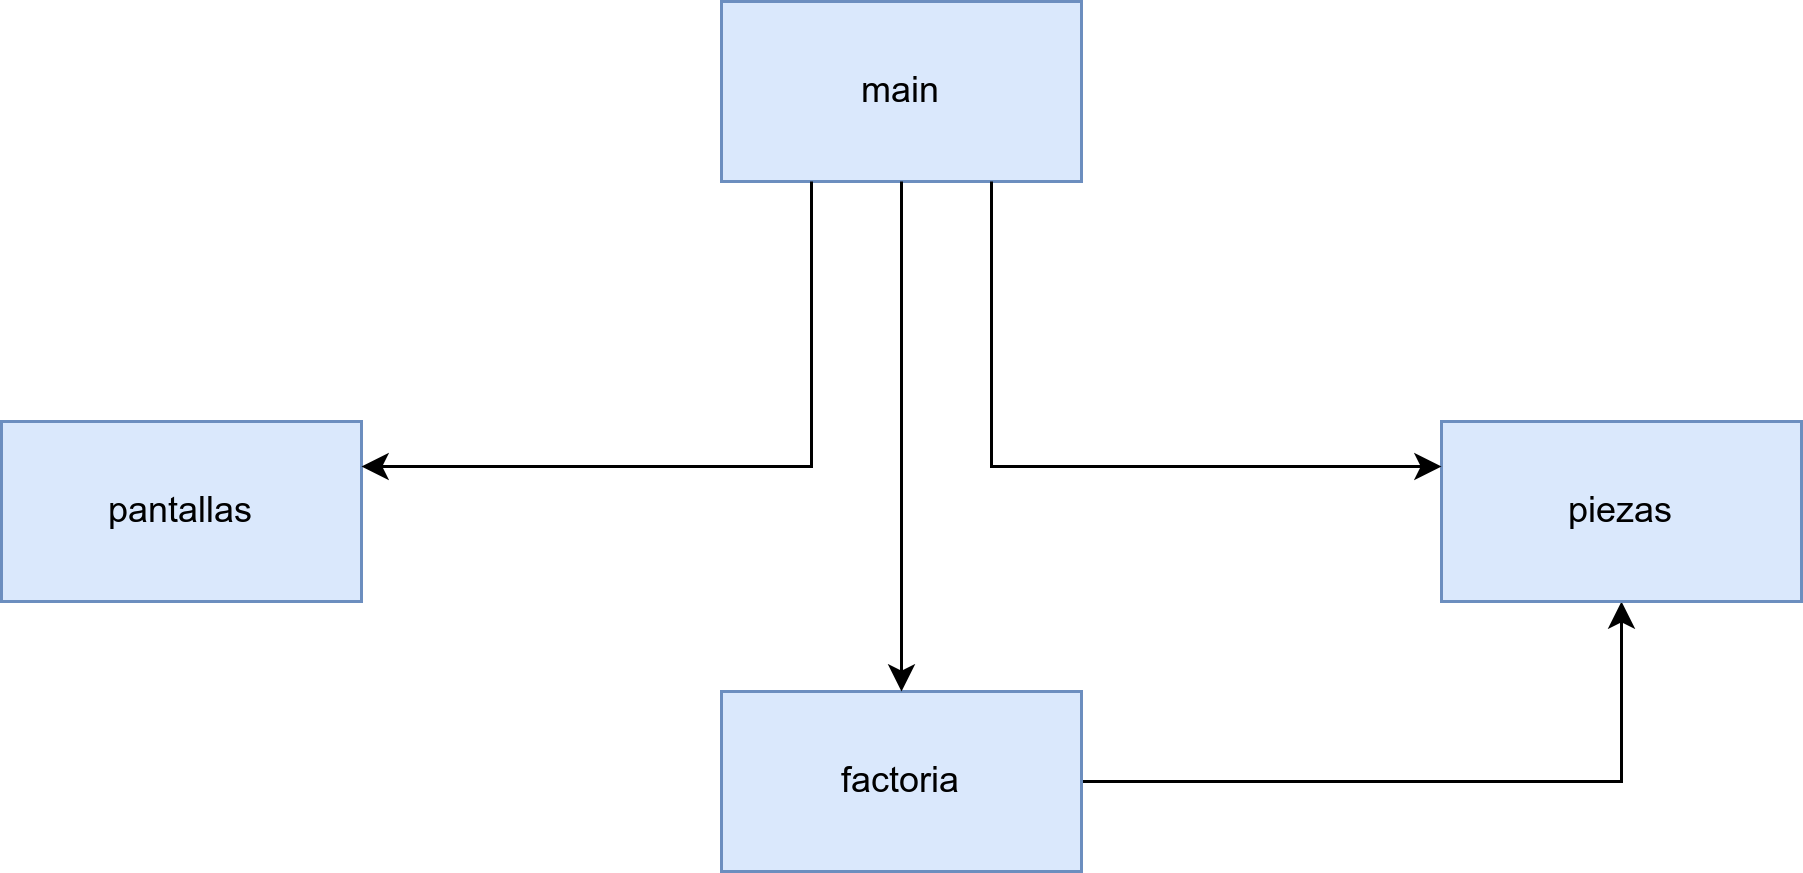
\includegraphics[width=\textwidth]{imagenes/paquetes.png}
        \caption{Diagrama de paquetes}
\end{figure}

\begin{figure}[H]
        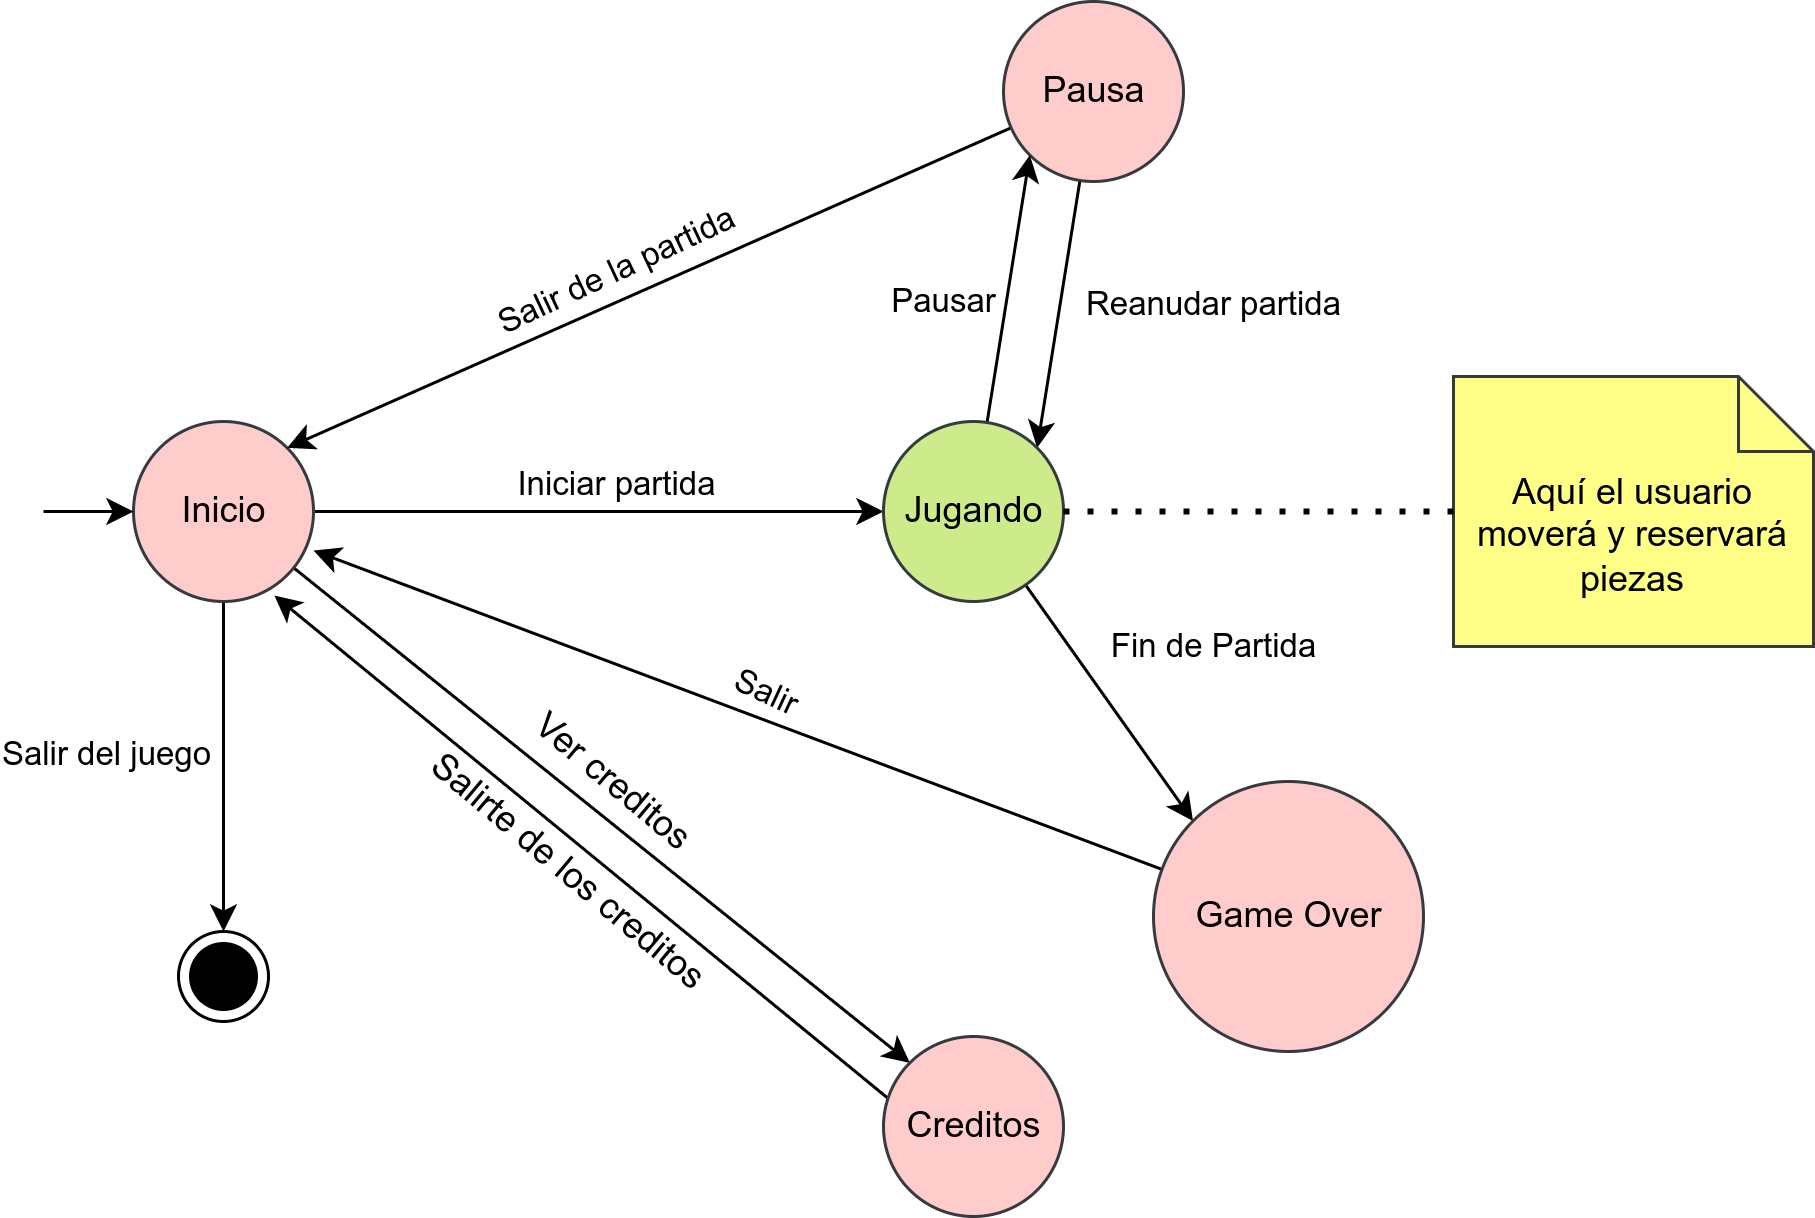
\includegraphics[width=\textwidth]{imagenes/estados.png}
        \caption{Diagrama de estados (autómata)}
\end{figure}

\subsection{Diagrama de clases}
\begin{figure}[H]
        \includegraphics[width=\textwidth]{imagenes/clase.png}
        \caption{Diagrama de clases}
\end{figure}

\section{Capturas de pantalla}
\begin{figure}[H]
  \begin{subfigure}{0.5\textwidth}
          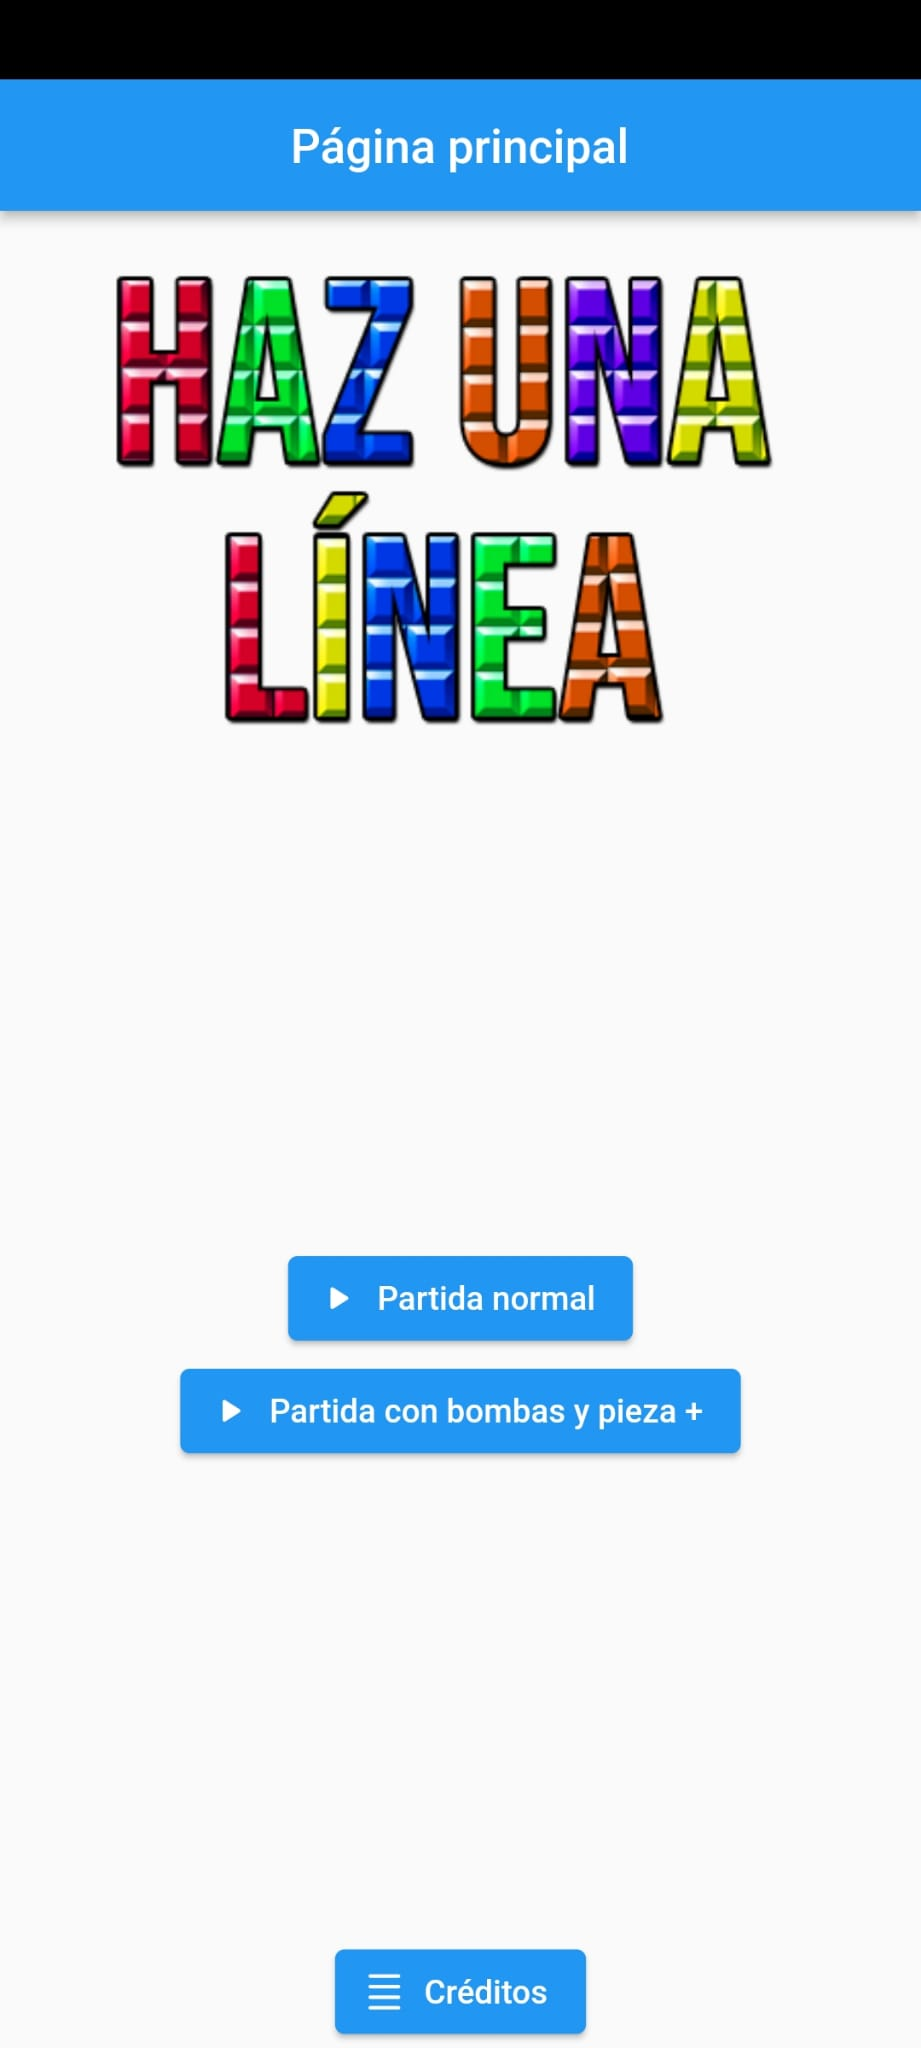
\includegraphics[width=\textwidth]{imagenes/captura7.jpeg}
          \caption{Modo claro}
  \end{subfigure}
  \begin{subfigure}{0.5\textwidth}
          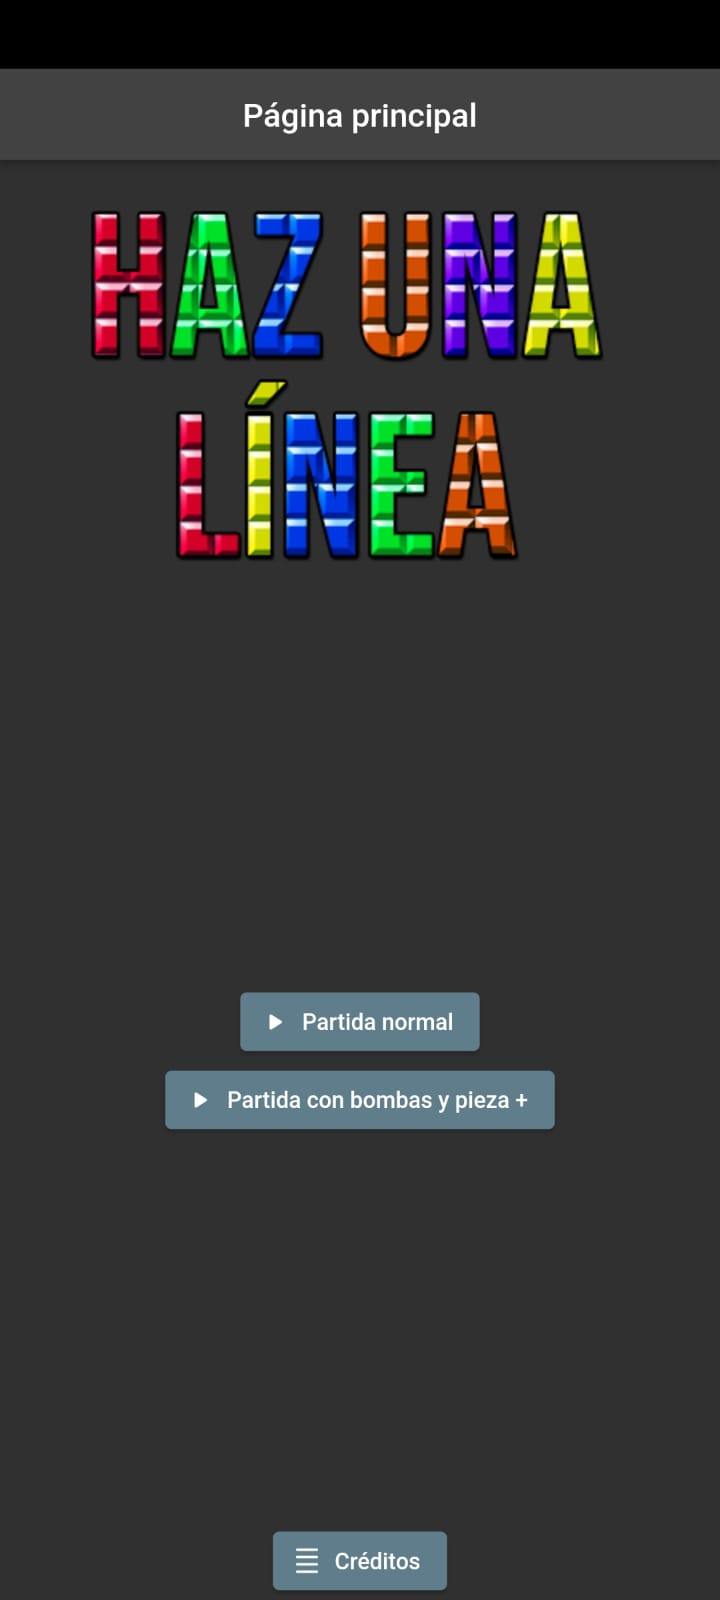
\includegraphics[width=\textwidth]{imagenes/captura1dark.jpeg}
          \caption{Modo oscuro}
  \end{subfigure}
  \caption{Pantalla de inicio de la aplicación.}
\end{figure}

\begin{figure}[H]
  \begin{subfigure}{0.5\textwidth}
          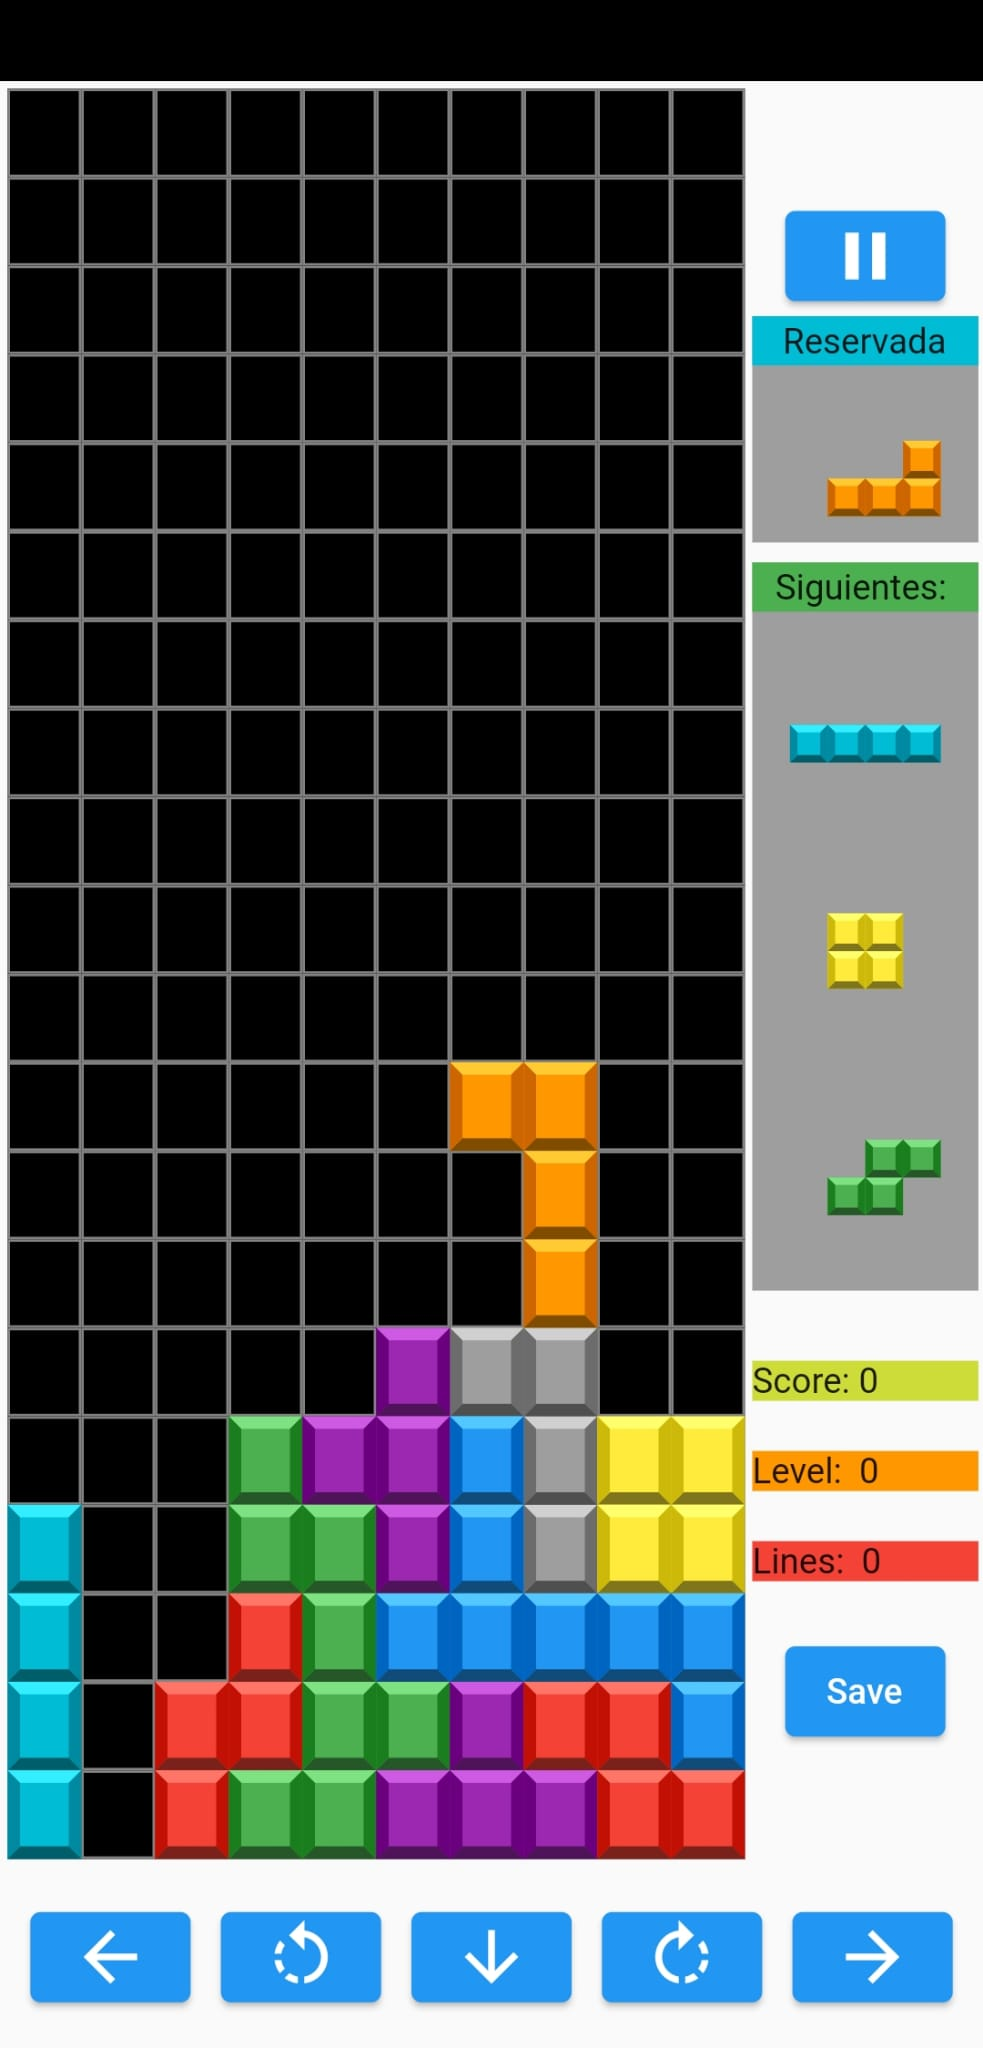
\includegraphics[width=\textwidth]{imagenes/captura1.jpeg}
          \caption{Modo claro}
  \end{subfigure}
  \begin{subfigure}{0.5\textwidth}
          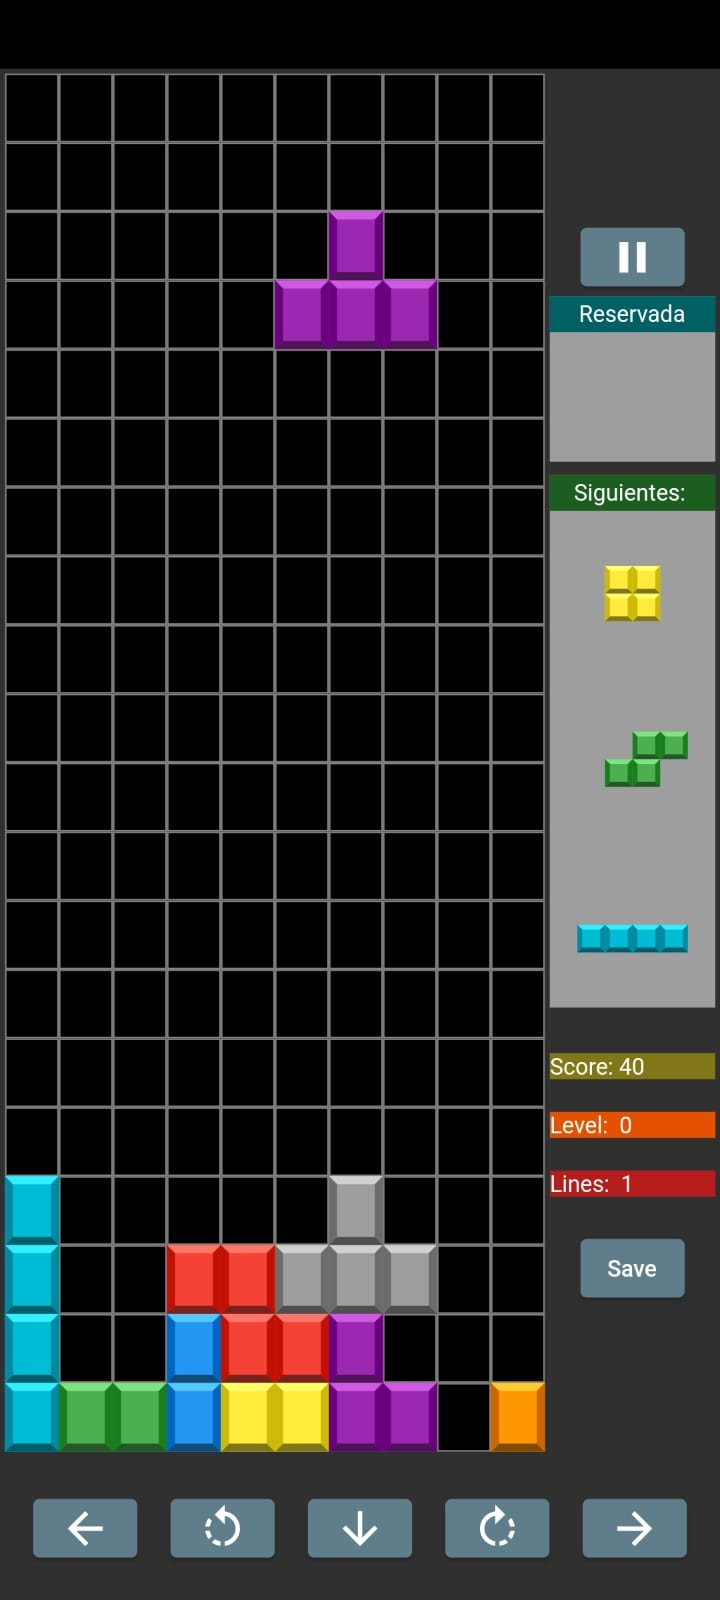
\includegraphics[width=\textwidth]{imagenes/captura2dark.jpeg}
          \caption{Modo oscuro}
  \end{subfigure}
  \caption{Ejemplo de tablero.}
\end{figure}

\begin{figure}[H]
  \begin{subfigure}{0.5\textwidth}
          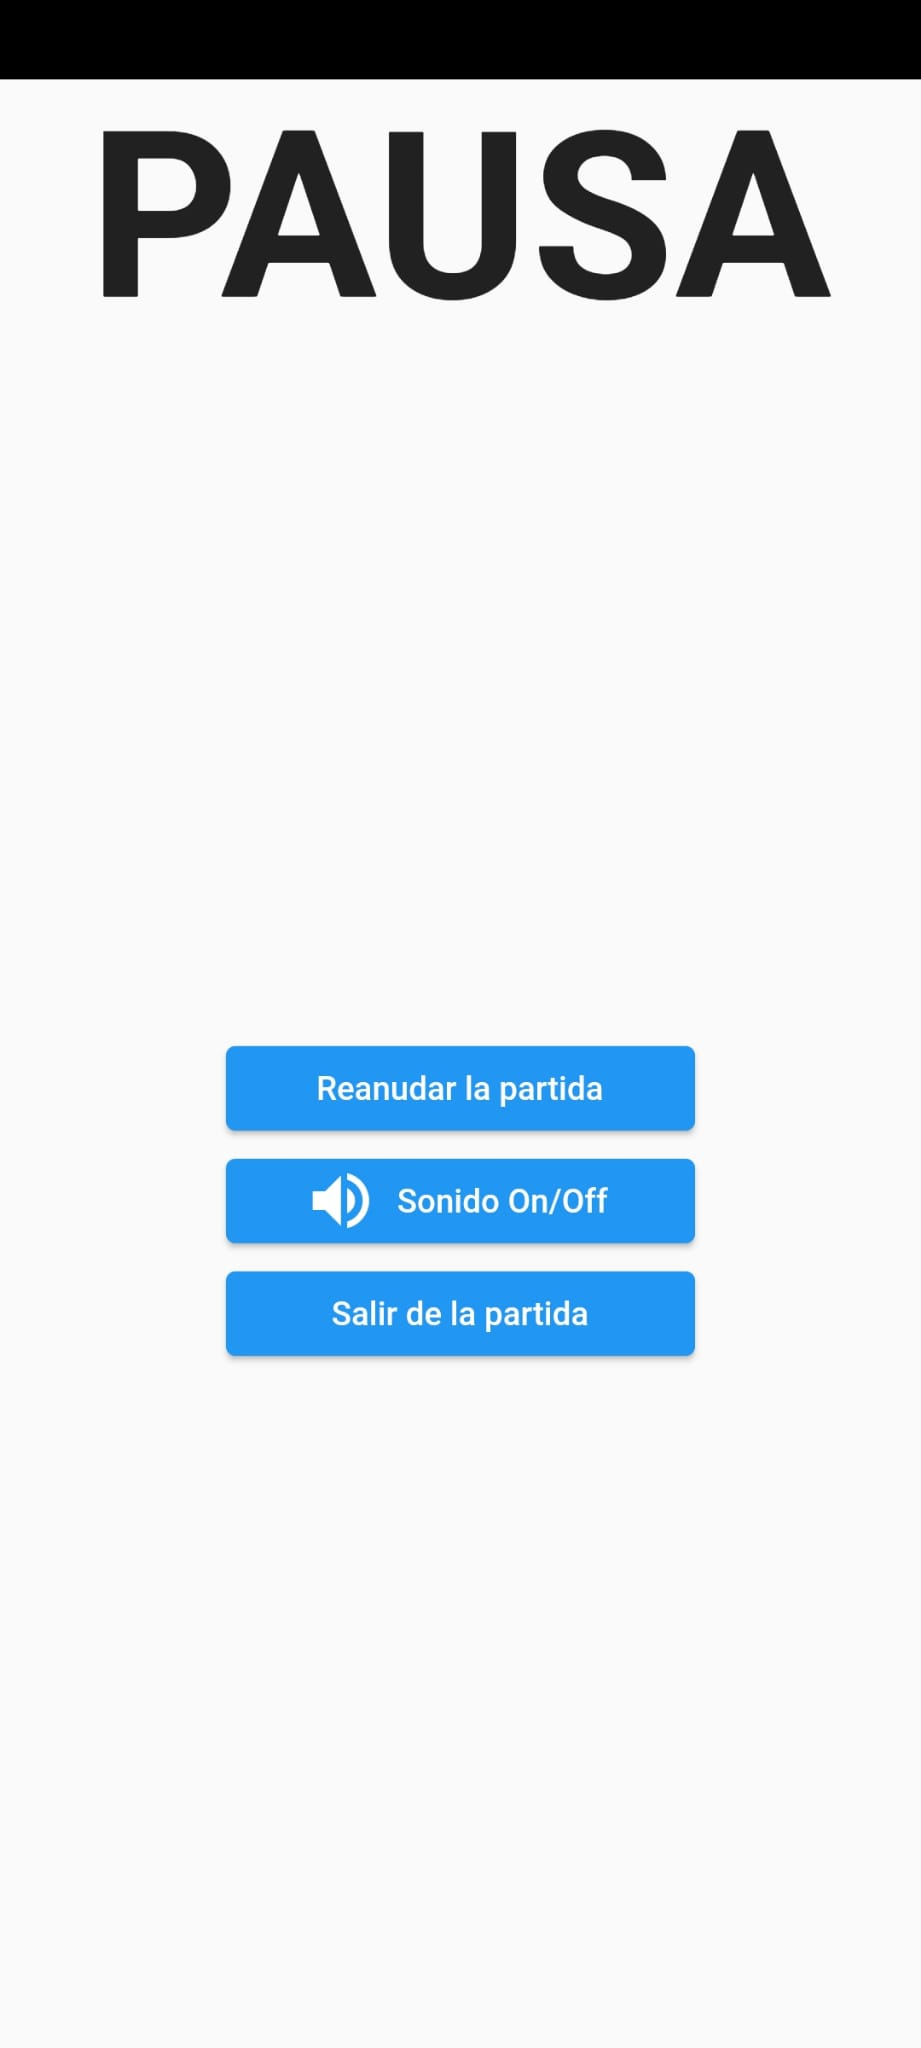
\includegraphics[width=\textwidth]{imagenes/captura6.jpeg}
          \caption{Modo claro}
  \end{subfigure}
  \begin{subfigure}{0.5\textwidth}
          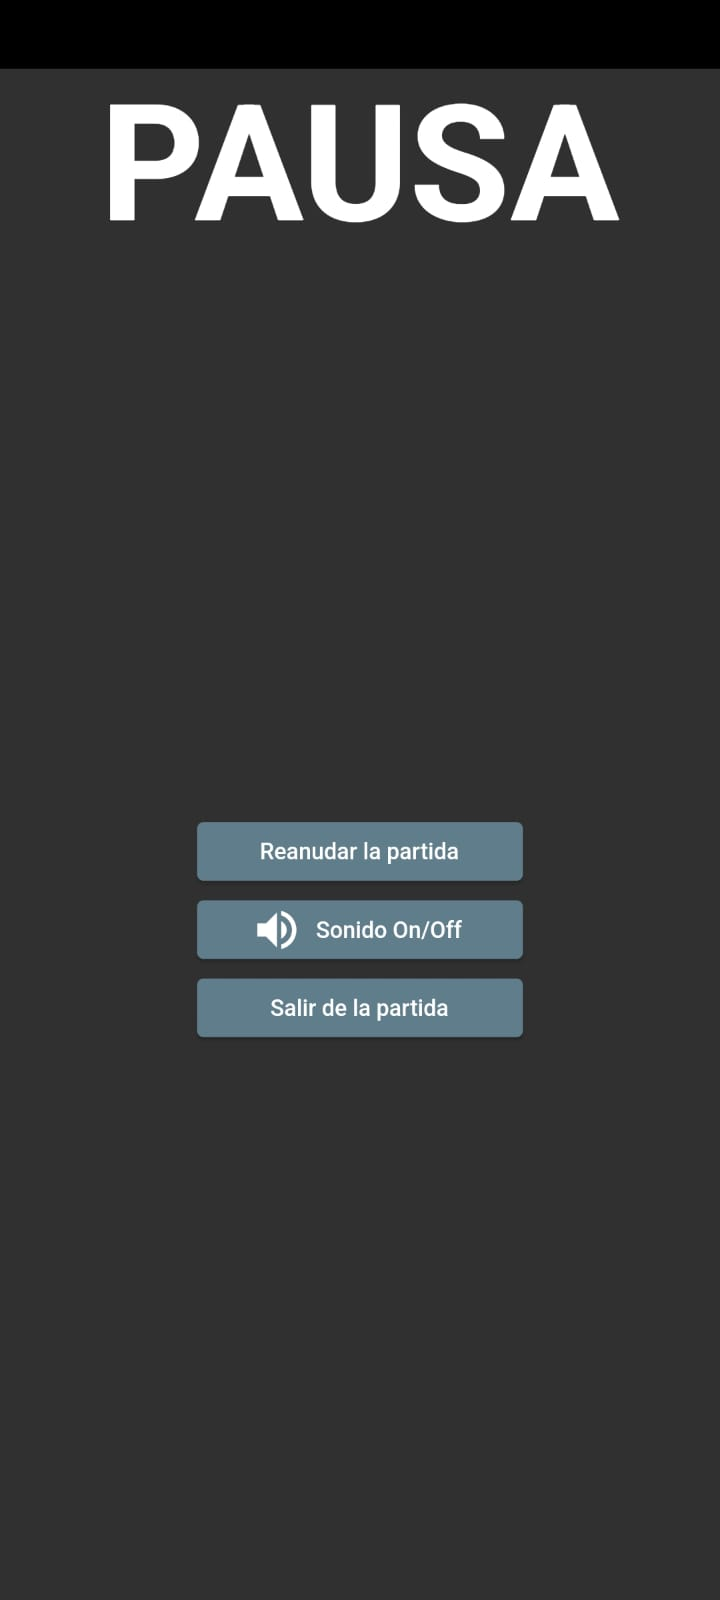
\includegraphics[width=\textwidth]{imagenes/captura3dark.jpeg}
          \caption{Modo oscuro}
  \end{subfigure}
  \caption{Pausa del juego.}
\end{figure}

\begin{figure}[H]
  \begin{subfigure}{0.5\textwidth}
          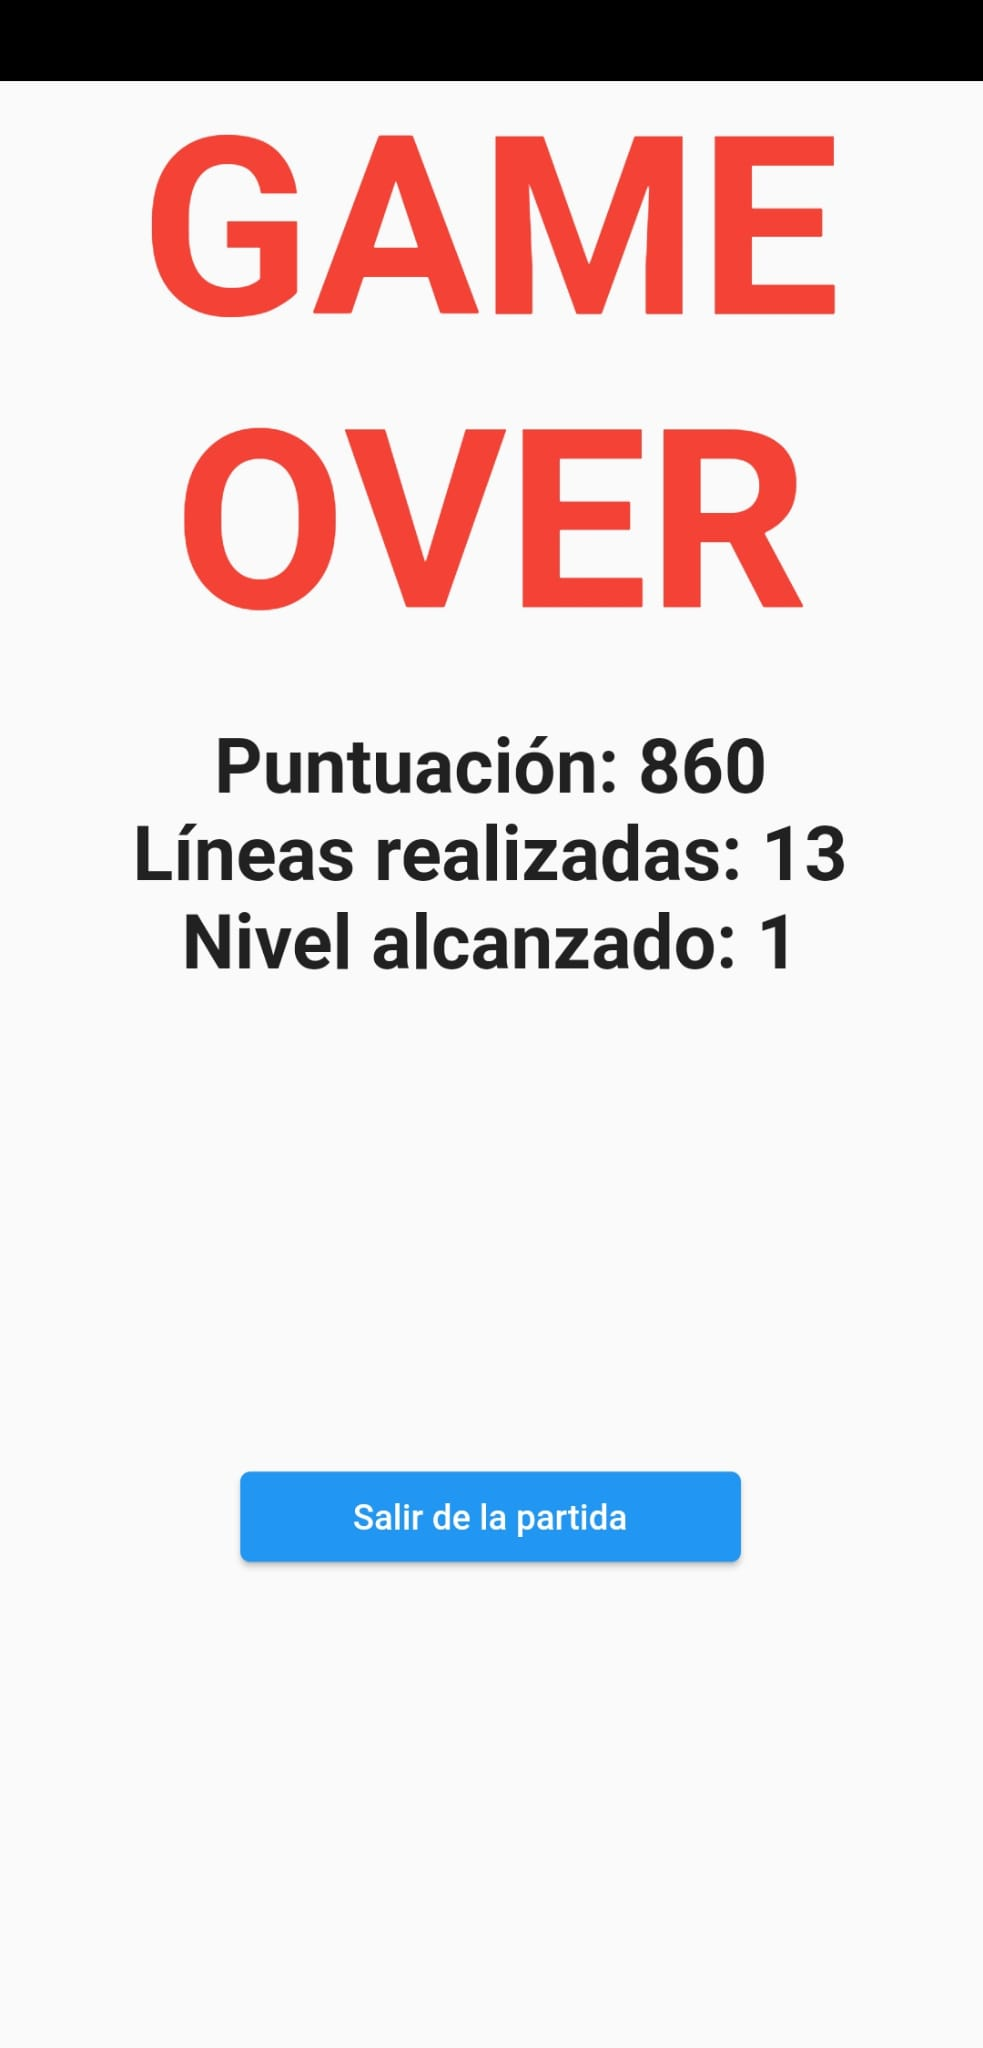
\includegraphics[width=\textwidth]{imagenes/captura4.jpeg}
          \caption{Modo claro}
  \end{subfigure}
  \begin{subfigure}{0.5\textwidth}
          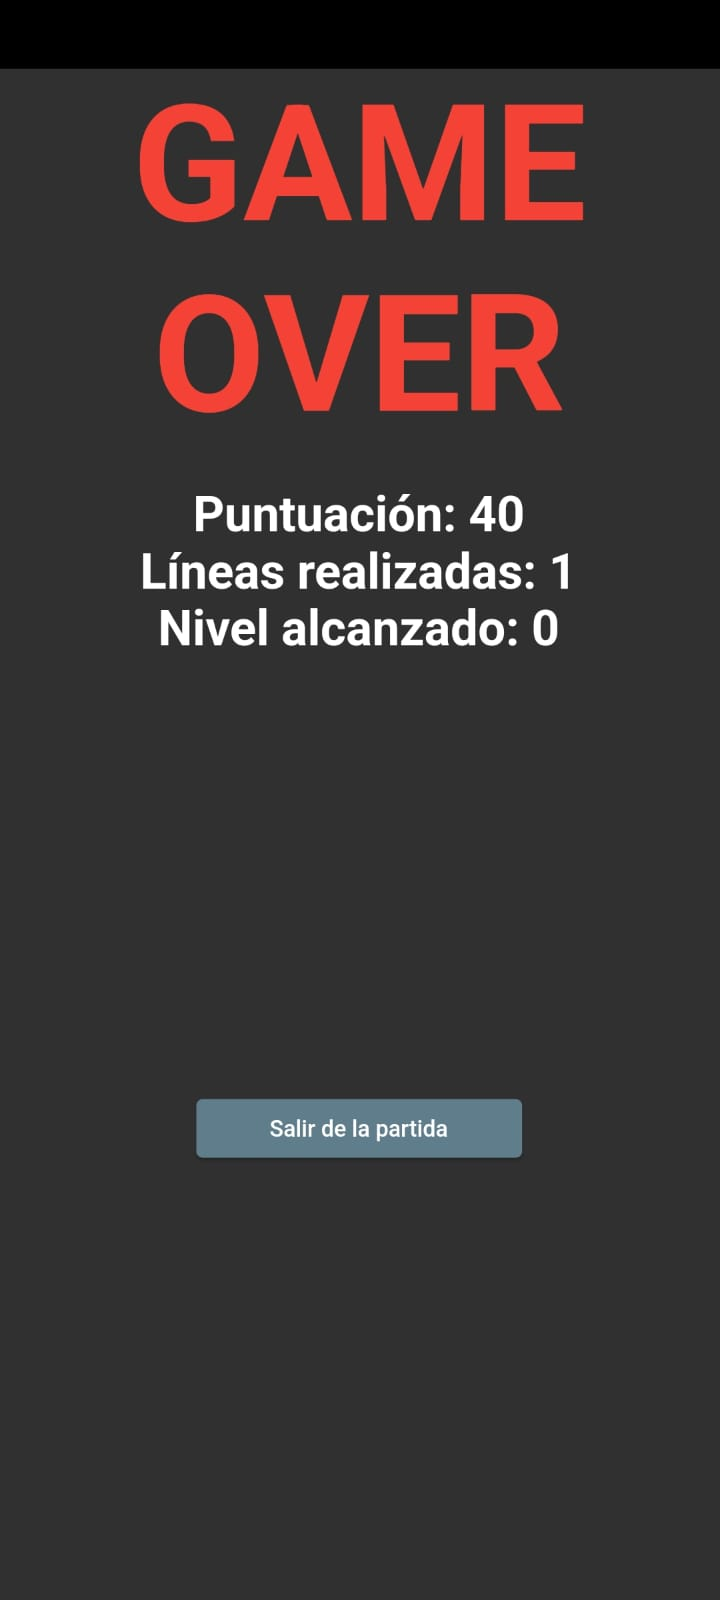
\includegraphics[width=\textwidth]{imagenes/captura4dark.jpeg}
          \caption{Modo oscuro}
  \end{subfigure}
  \caption{Pantalla de Game Over}
\end{figure}


\end{document}
